\chapter{Related Work}
\label{cha:related-work}

This chapter examines prior research on changing behavior through information technology and related systems. First I cover research in energy feedback, which forms the foundation for participants understanding of their energy use, followed by a description of the practical methods of recording electricity data. Next, I cover research into motivations for pro-environmental behavior, and techniques that have been demonstrated to foster that behavior. The Kukui Cup uses these techniques to build a persuasive game experience for participants, and the following sections cover the design of environmentally persuasive systems, and game design. An important goal of the Kukui Cup pedagogy is to increase the energy literacy of participants, so the topic of energy literacy is covered next. The final two sections review systems related to the Kukui Cup, and research on dorm energy competitions.


\section{Energy Feedback}
\label{sec:energy-feedback}

As Lord Kelvin is famously reputed to have said, ``If you can not measure it, you can not improve it.'' In the case of electricity usage, for many people the only feedback they receive is a monthly bill detailing the number of kilowatt-hours used over the course of the last month. Ed Lu of Google analogizes this as if there were no prices items at the grocery store, and shoppers were just mailed a bill at the end of the month~\cite{Helft2008Googles-Energy}. Office workers or dormitory residents might never see any feedback on how much electricity they are using!

Feedback systems display the consumption of a resource (such as electricity) to the user, usually in real time. Darby provides a detailed survey of studies on electricity feedback systems from the past 3 decades \cite{darby-review-2006}. The survey of 20 studies finds that, on average, the introduction of a direct (real-time) feedback system leads to reductions of energy usage ranging from 5-15\%. Feedback systems providing historical data (such as those provided with billing statements) are not as effective (0-10\% reductions), but can be useful for assessing the impact of efficiency measures such as improved insulation or a more energy efficient appliance, since those savings accumulate over time.

Darby found that ``consumption in identical homes, even those designed to be low-energy dwellings, can easily differ by a factor of two or more depending on the behaviour of the inhabitants.'' This finding demonstrates the significant potential to curb energy usage through changes in individual's behavior.

Another survey of energy feedback was conducted Faruqui et al., looking at 12 utility pilot programs that installed in-home displays with near-realtime feedback \cite{Faruqui09}. They found that customers that actively used the display averaged a 7\% reduction in energy usage, while those pilot programs that included pre-paid electrical services reduced their energy usage by 14\%. The sustainability of the energy reduction is unclear based on the pilot studies since they were of limited length. The authors believe it is unknown whether the residents of homes with displays will acclimate to the display and cease to use it to reduce their energy usage.

Foster and Mazur-Stommen surveyed nine large-scale, real-time feedback pilot studies conducted recently in the US, UK, and Ireland~\cite{Foster-2012}. Energy savings in the studies ranged from 0--19.5\%. The 19.5\% savings occurred in a multi-year study in Northern Ireland that combined real-time feedback with pre-payment of electrical service. The addition of pre-payment (which is uncommon in other areas) is likely the factor that increased the conservation. The average energy savings was 3.8\% (excluding the Northern Ireland pilot), with two studies finding no aggregate effect of real-time feedback. Some studies found that certain households saved up to 25\%, and Foster and Mazur-Stommen refer to these as ``cybernetically sensitive'' households. They postulate that these cybernetically sensitive households are particularly motivated by feedback in energy use. These households appear to cut across demographic lines, so identifying them in advance will require further research. The persistence of savings across the pilots was mixed. Some pilots found that electricity savings increased over time, possibly due to learning about energy consumption habits. Those pilots that tested persistence found that some savings persisted during the pilot, except for one that returned to zero after four weeks. The persistent savings fell from higher initial savings over time. Foster and Mazur-Stommen identify five factors that can affect energy savings from real-time feedback:

\begin{itemize}
	\item ``a `sensitivity' towards real-time energy consumption feedback;
	\item the design of and content provided by feedback devices, and the degree to which these facilitate the tasks that consumers want to accomplish through feedback;
	\item the installation process and reliability of feedback devices;
	\item engagement with feedback, which is both confounded and encouraged by dynamics within the household; and
	\item the degree to which learning and habit formation take place.''
\end{itemize}

They found that the infrastructure overhead of obtaining real-time feedback (meter cost, installation) was high compared to other energy conservation techniques, though it would likely go down as more households are served. From a utility perspective, it might not be a good investment outside of the cyber-sensitive households. They also point out that research on the means by which energy is conserved in the household is still very limited, and suggest ethnographic research methods might be helpful in this regard.

Darby also points out that while feedback is critical for energy conservation behaviors, feedback alone is not always enough \cite{darby-2000-making-it-obvious}. Other factors that lead to higher rates of energy conservation include contact with an advisor when needed, and training and social infrastructure.

\begin{figure}[htbp]
	\centering
		\includegraphics[width=\textwidth]{current-energy-website}
		\caption{View of LBNL's Current Energy Web Site on December 15, 2004}
		\label{fig:current-energy-website}
\end{figure}

During California's energy crisis in 2000 and 2001, Lawrence Berkeley National Laboratory created a web site that graphed data from utility organizations \cite{Bartholomew2008Current-Energy}. The graphs showed consumer demand for electricity (actual and forecast), and the utilities' generation capacity (see \autoref{fig:current-energy-website} for an example graph). Darby reports anecdotal evidence that people viewing the graphs changed their electricity usage based on the data \cite{darby-review-2006}.

Ecotricity, a renewable energy utility in the UK, has developed a grid-level feedback system. The Ecotricity website provides a real-time dashboard that displays the types of energy sources used to power the UK grid (fossil fuels, nuclear, and renewable) and the overall carbon intensity of the grid in g\COtwo per \kWh as shown in \autoref{fig:ecotricity-dashboard}. The carbon intensity display is made actionable through a traffic light visualization that is green when the grid is emitting less carbon and red when it emits more carbon. 

\begin{figure}[htbp]
	\centering
		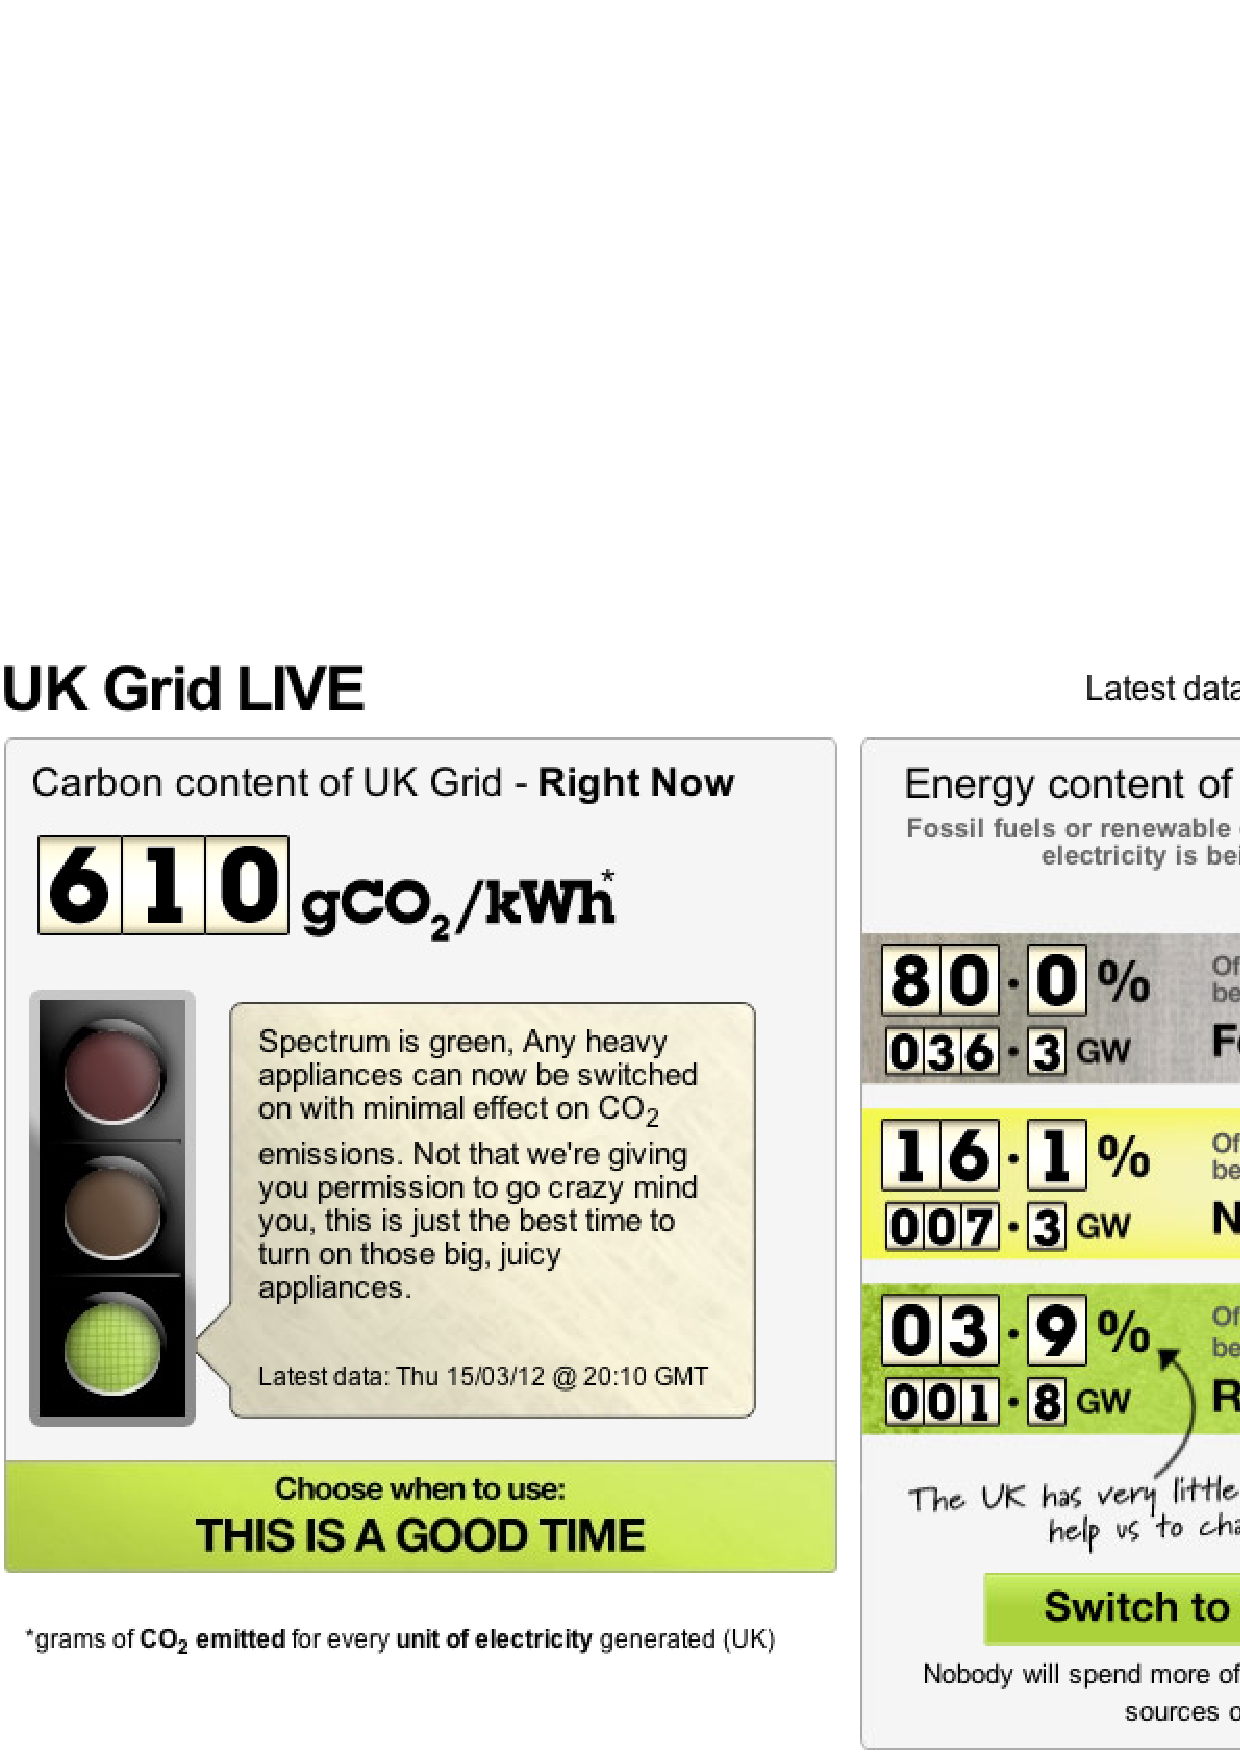
\includegraphics[width=\textwidth]{ecotricity-dashboard}
		\caption{Ecotricity's live UK Grid dashboard}
		\label{fig:ecotricity-dashboard}
\end{figure}

There is also evidence that just the knowledge that one is being monitored can cause one to consume fewer resources. A group of researchers simulating a mission to Mars or the Moon in the Canadian Arctic for four months tracked the crew members' water usage \cite{Bamsey2008FMARS}. Water usage was monitored via automated meters during the entire mission, but during certain multi-day study periods, crew members were also required to manually log their water usage at the point of use. The authors found that water usage was 10\% less during these study periods. The reduced water usage could be due to the knowledge that the usage was being examined more closely, or perhaps the extra effort required to manually record their water usage led to crew members reducing non-essential water use (see \autoref{sec:ecoisland} for another possible benefit to manual data collection).

\begin{figure}[htbp]
	\centering
		\subfigure[Device itself]{\label{fig:thighmaster-device}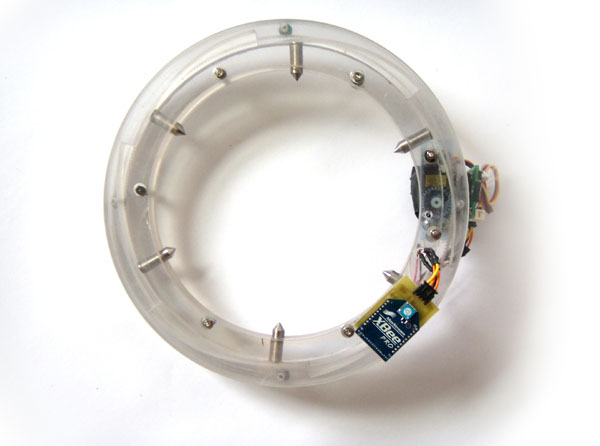
\includegraphics[height=2.5in]{thighmaster-alone}}
		\subfigure[As worn on leg]{\label{fig:thighmaster-leg}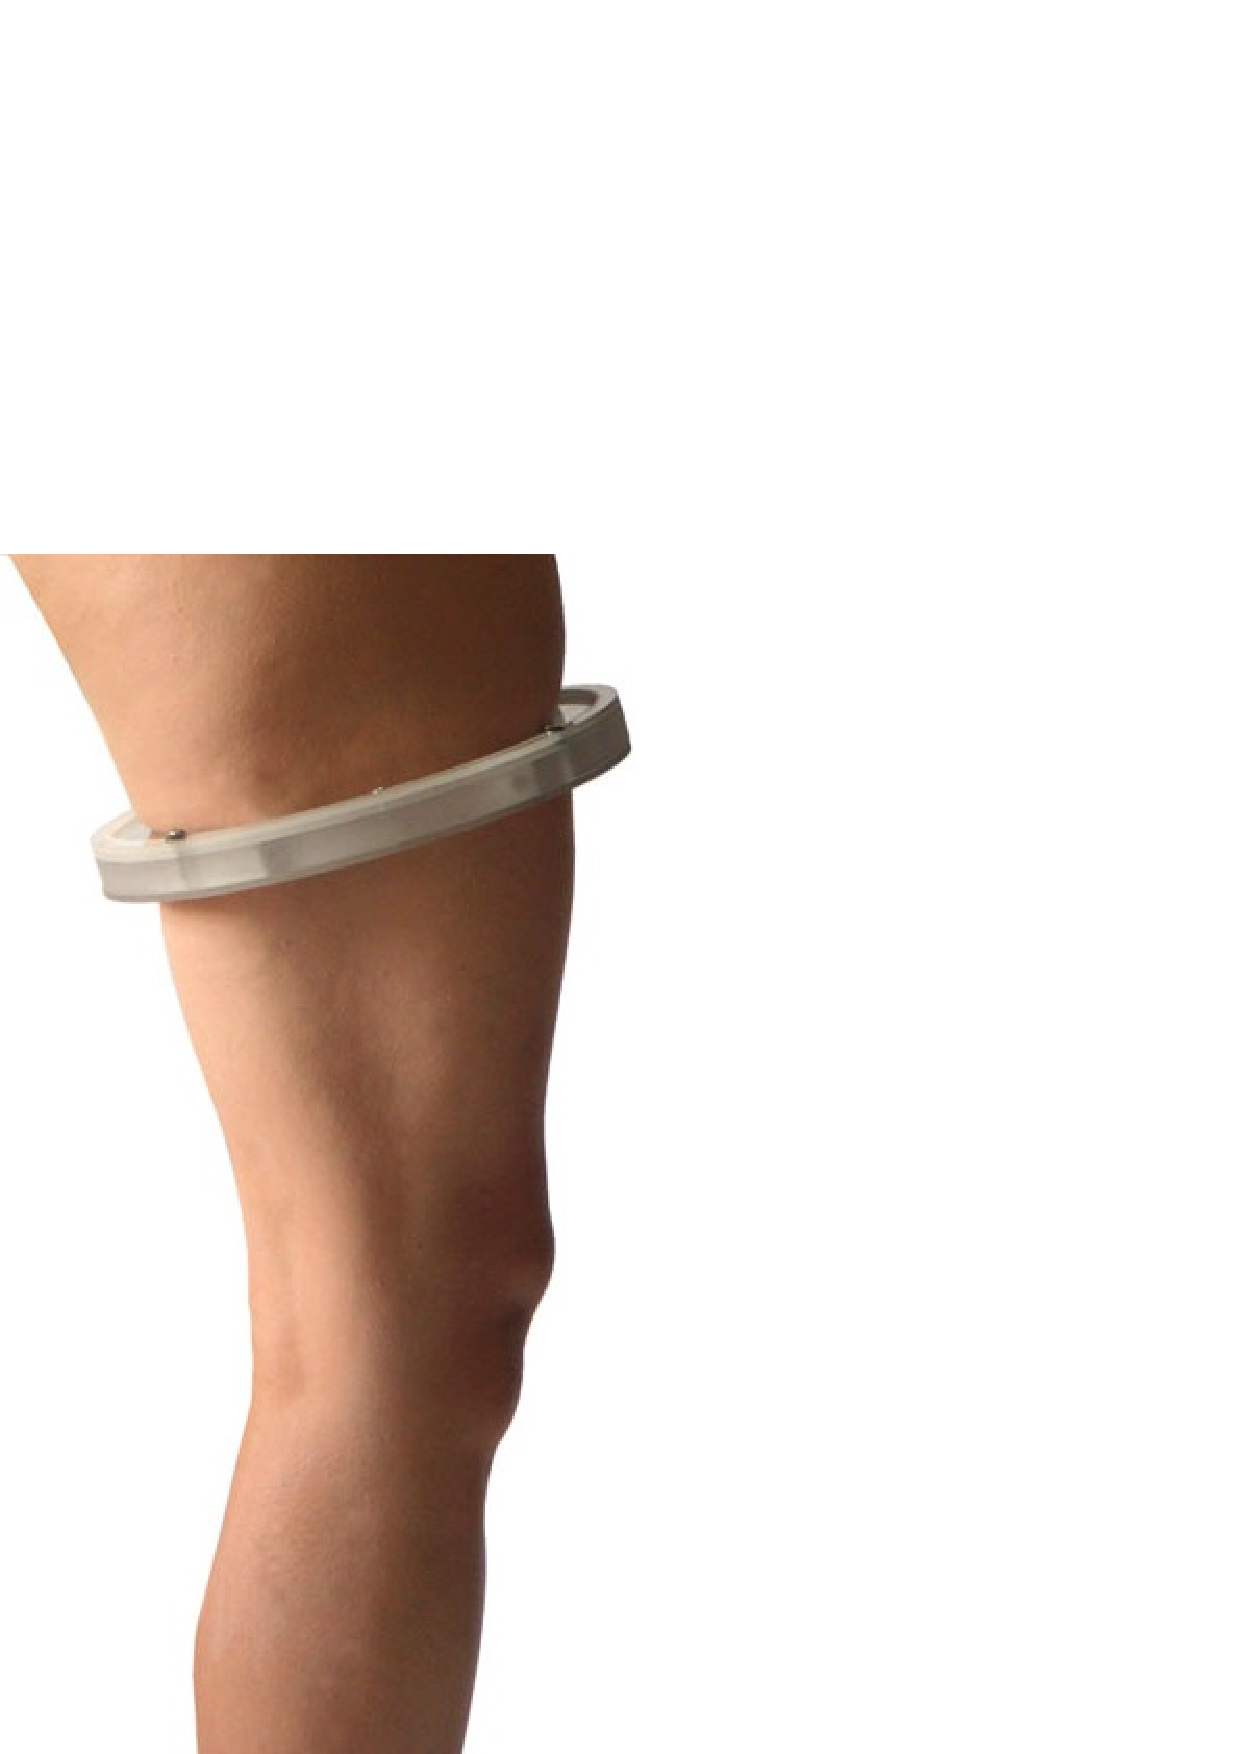
\includegraphics[height=2.5in]{thighmaster-leg}}
		\caption{Thighmaster energy feedback mortification device}
		\label{fig:thighmaster}
\end{figure}

R\"{u}st has implemented an extreme energy feedback system called the Thighmaster \cite{Rust2008Thighmaster-web}. Inspired by the cilice (a small metal garter with inward facing spikes) worn by some members of the Catholic Opus Dei organization as part of a practice of mortification, the Thighmaster is a ``techno-garter'' that pokes the wearer with spikes when their actions are not environmentally responsible (as defined by R\"{u}st), see \autoref{fig:thighmaster} for a depiction of the device. Specifically, the Thighmaster communicates wirelessly with electricity usage sensors and a human speech sensor that monitors whether the user speaks with their plants. While more of a demonstration, the Thighmaster shows the complex emotions involved in people's reactions to climate change. It goes without saying that being pierced by spikes is unlikely to be a viable energy feedback mechanism for most users.

Energy feedback was a core element of the Kukui Cup system. Feedback provides awareness of energy use that participants in student housing have likely never experienced before, and provides verification to participants that behavior changes can change energy use. Many studies have shown that providing energy feedback leads to some degree of energy conservation, so feedback is another useful component in the Kukui Cup system. However, feedback is alone is not necessarily successful, as two studies that resulted 0\% energy reduction demonstrate. Energy data needed to provide feedback to participants is also necessary for both the scoring of the energy competition and as one means of evaluating the impact of the system.


\section{Electricity Metering}

Electricity metering systems can be broken down into two types: plug load meters that measure the electrical load directly plugged into them, and panel energy meters that measure the electrical usage of an entire distribution panel (which might cover an entire small building, or a floor of a larger building). Both typically provide a real-time display of electricity usage, and some sort of historical total (usually in kilowatt hours).

\subsection{Plug Load Meters}
\label{sec:plug-load-meters}

The Kill-A-Watt is an example of an inexpensive plug load meter \cite{kill-a-watt}. It is designed to be plugged into a wall outlet, and the load is then plugged into the Kill-A-Watt. An LCD display shows the current voltage, current, power, frequency, power factor, and cumulative energy used since the unit was plugged in. The Kill-A-Watt provides an easy way to determine how much electricity a particular appliance (or set of appliances if connected via a power strip) uses. The manufacturer claims the Kill-A-Watt is accurate to within 0.2\%. There are several drawbacks to the Kill-A-Watt. Because of its shape, it generally obscures both of the outlets commonly found on a wall outlet in the US, preventing the second outlet from being use while measurement is taking place. The load must be plugged in via the Kill-A-Watt, so that means that the user must disconnect the load from power at least momentarily, which can be inconvenient for some loads (computers, refrigerators, etc.). The Kill-A-Watt also has no facility for exporting the data it collects, and if power is lost for any reason, the data collected will be lost as well.

LeBlanc attempted to address the issue of data collection with his work on recording device-level power consumption \cite{leblanc-2007}. He developed a sensor that sits between the load and the wall outlet, like the Kill-A-Watt. The sensor records electricity usage, and transmits the data wirelessly using the ZigBee protocol to a base station. Details on how to construct the wireless power monitor can be found at the author's personal website \cite{LeBlanc2008power-mon-howto}. This system solves the problem of automated data collection, but still requires the load to be unplugged before monitoring. It also faces the problem of all plug-load meters, which is that it can only monitor what it is connected to, therefore it is unsuitable for providing a comprehensive picture of electricity usage in a building or floor.

\subsection{Panel Meters}
\label{sec:panel-meters}

The Energy Detective TED Model 5000 is a panel electricity meter from Energy, Inc \cite{the-energy-detective}. TED consists of three components:

\begin{itemize}
	\item a Measuring Transmitting Unit (MTU), which is connected directly to the incoming power lines at the circuit breaker box
	\item a Gateway that receives data from the MTU through the electrical wiring of the home, stores it, and makes the data available via HTTP using an Ethernet connection
	\item a handheld, wireless display unit that provides a continuously updated display of power usage sent via the Zigbee protocol from the Gateway.
\end{itemize}

The MTU uses current transformers, which clamp over the incoming power cables, and measure the amount of current being transmitted over them. Because the transformers clamp over the existing cables, there is no need to alter the existing wiring. The instantaneous power consumption can be computed using the current data combined with the utility voltage. These data are transmitted to the display unit through the building's electrical wiring.

The display unit receives the instant power consumption data from the Gateway unit every few seconds. The power consumption data can be displayed in real time in kilowatts or dollars (after the user enters pricing data). It can also track historical consumption, peak usage, and project usage for the rest of the month based on historical usage. The Gateway unit provides a detailed web interface to the power data for computers inside the home, and can be configured to upload data to Google PowerMeter (\autoref{sec:google-powermeter}) every 15 minutes. Energy Inc makes an XML API available for developers who wish to use the data directly. TED appears to be the lowest cost option for whole home electricity monitoring with data recording and Internet accessibility.

While panel energy meters provide only building-wide usage data, users can use the real-time display to figure out the impact of particular uses as air conditioning through trial and error experimentation. Parker et al.\ describe a protocol for using a household-wide meter and a circuit breaker panel to localize the energy usage in a home \cite{Parker2006How-Much-Energy}. All the breakers are turned off, and then turned on one at a time while recording data from the electrical meter. In 2--4 hours, users were able to generate a spreadsheet mapping the electricity usage in their homes.

\subsection{Building Energy Displays}
\label{sec:building-energy-displays}

Another type of electricity usage monitoring is building energy displays, which monitor electricity usage for an entire building (usually non-residential, such as a school or office building) and display the usage information in some public area such as a lobby. Green TouchScreen \cite{greentouchscreen} and Building Dashboard \cite{building-dashboard} are examples of this type of product. These devices aim to make building occupants aware of the overall environmental impact of the building, which is something usually invisible to the occupants. Some systems make the displays available via the web so that users can view the information from their desk as well as the lobby. The displays often provide  information beyond just electricity usage, such as water or natural gas usage, and may display the usage in units other than kWh, such as number of incandescent light bulbs lit or hours of TV watching. Beyond their potential utility in helping building occupants to reduce their energy usage, informative displays can be used to get points toward Leadership in Energy and Environmental Design (LEED) certification for a building.


\subsection{Metering Summary}

While plug load meters are helpful since they can provide power and energy data about a single device, using them for energy metering in the 2011 Kukui Cup is not appropriate for several reasons: it would require approximately 2800 meters to cover all in-room outlets, plug load meters cannot track overhead lighting use, they would be easy to circumvent to reduce reported energy use, and per-outlet energy data raises important privacy issues that would complicate the competition. We did make use of plug load meters for the room energy audit activity, where participants used the meters to determine the power use of each devices in their room.

As will be discussed in \autoref{sec:meter-selection}, the Kukui Cup used panel meters installed on each floor of the residence halls for energy data collection. No building energy displays were deployed as part of the 2011 Kukui Cup, due to the cost of displays and the logistics of installing displays in a vandal and theft-proof manner.


\section{Motivation}

In encouraging individuals to change their energy use behaviors, it is worthwhile to examine research on motivations for behavior. This section starts with a discussion on intrinsic versus extrinsic motivations, followed by an alternative multifaceted theory of motivation. Then I cover research on specific motivations for environmentally responsive behaviors, ending with a summary of motivation research as it applies to the Kukui Cup.


\subsection{Intrinsic and Extrinsic Motivation}

One area of research into human motivations characterizes motivations as either intrinsic or extrinsic: intrinsic motivations are those behaviors where the activity is its own reward, whereas extrinsic motivations are external rewards provided for a particular desired behavior. A great deal of research has been conducted on the relationship between these two types of motivation. One particular concern is over the possibility that provision of external rewards (extrinsic motivators) might reduce intrinsic motivation for tasks. For example, subjects asked to draw pictures and then rewarded with money or candy might later be less likely to draw pictures in the absence of rewards, which is interpreted as a reduction in intrinsic motivation for drawing. This effect of extrinsic rewards reducing intrinsic motivation is termed \emph{undermining}. There is debate in the research community as to whether undermining is a common effect, or uncommon and of little practical implication. Deci et al.\ performed a meta-analysis of 128 studies of extrinsic rewards on intrinsic motivation, and found pervasive evidence that extrinsic rewards did in fact reduce intrinsic motivation~\cite{Deci1999}. Cameron et al.\ performed a later meta-analysis and found no effect or a positive effect of extrinsic rewards on intrinsic motivation in many cases.~\cite{Cameron2001} Specifically, they found intrinsic motivation towards low-interest tasks was improved by the measure of free choice intrinsic motivation (time spent on tasks after rewards are removed) and unchanged in self-reported task interest. When rewards are provided for performing better than others, studies showed significant increases in free choice and task interest. Cameron et al.\ note that the magnitude of the impacts, both positive and negative are generally small.


\subsection{Multifaceted Motivation}

While the intrinsic/extrinsic dichotomy is a popular framework for studying motivation, others find it highly problematic. Reiss critiques the collapsing all motives into two categories as a gross oversimplification~\cite{Reiss2012}. He finds the use of behavioral measures of intrinsic motivation (such as recording the activities of children playing freely) as inferior to self-reports of motivation, and questions the reliability of such behavioral measures. Reiss instead proposes a multifaceted theory of motivation that he calls the \emph{theory of 16 basic desires}~\cite{Reiss2004}. These 16 desires or human needs are summarized in \autoref{tab:16-basic-desires}. While these desires are claimed to be universal, each individual will aim for higher or lower degrees of each type of motivation and these differences are the significant point of the theory. Reiss and collaborators have developed the Reiss Motivation Profile to assess which areas an individual is most motivated by, which has been validated in areas including sports, careers, and spirituality.


\begin{table}[htbp]
	\centering
		\begin{tabular}{| l | l |}
			\hline
Motive name & Motive \\ \hline
Power & Desire to influence (including leadership; related to mastery) \\ \hline
Curiosity & Desire for knowledge \\ \hline
Independence & Desire to be autonomous \\ \hline
Status & Desire for social standing (including desire for attention) \\ \hline
Social contact & Desire for peer companionship (desire to play) \\ \hline
Vengeance & Desire to get even (including desire to compete, to win) \\ \hline
Honor & Desire to obey a traditional moral code \\ \hline
Idealism & Desire to improve society (including altruism, justice) \\ \hline
Physical exercise & Desire to exercise muscles \\ \hline
Romance & Desire for sex (including courting) \\ \hline
Family & Desire to raise own children \\ \hline
Order & Desire to organize (including desire for ritual) \\ \hline
Eating & Desire to eat \\ \hline
Acceptance & Desire for approval \\ \hline
Tranquility & Desire to avoid anxiety, fear \\ \hline
Saving & Desire to collect, value of frugality \\ \hline
		\end{tabular}
	\caption{16 basic human desires, adapted from Reiss, table 1~\cite{Reiss2004}}
\label{tab:16-basic-desires}
\end{table}


\subsection{Motivation of Environmentally Responsible Behaviors}

De Young investigated the motives behind individual's environmentally responsible behaviors (ERBs) through a series of surveys \cite{Young:2000fv}. Traditionally, the motives invoked by researchers attempting to promote ERB were constrained to material incentives or disincentives and altruistic reasons. The problem with incentives is that they ``needed constant reintroduction to remain effective and they proved to be less reliable than we had hoped''. Incentives can initiate ERB, but people's behavior changes back when the incentives end, and even continuing incentives can have low reliability.

De Young also describes some of the pitfalls that can be encountered in motivating ERB, such as psychological reactance, where people do the opposite of the ERB they are being asked to undertake. Even those initiating the behavior changes can be negatively impacted. De Young describes some initiators experiencing feelings of contempt for those whose behavior they are trying to change, and also contempt for themselves.

Self-interest is generally considered the cause of environmental problems: ``focusing solely on short-term individual or familial gain to the exclusion of long-term societal or environmental benefits''. De Young, however, suggests that self-interest can be a solution to environmental problems. He distinguishes self-interest from selfishness: self-interest meaning each individual is responsible for getting their own needs met. De Young believes that intrinsic satisfaction is a better way to motivate ERB, as people find that ``certain patterns of behavior are worth engaging in because of the personal, internal contentment that engaging in these behaviors provides.''

Based on 9 different studies of ERB across different populations and environmental focuses, De Young found 3 intrinsic satisfactions:
\begin{enumerate}
	\item ``satisfaction derived from striving for behavioral competence''
	\item ``frugal, thoughtful consumption''
	\item ``participation in maintaining a community''
\end{enumerate}

Competence involves the enjoyment in completing tasks and solving problems. Frugality is enjoyment from the ``careful stewardship of finite resources''. Participation is the enjoyment from participating in community activities such as sharing news and collaborating with others toward a shared goal.

While attitudes and norms can lead to behavior change, people also need tools and guidance to realize this change. As De Young puts it, ``without considering these variables, we make the error of assuming that once people know what they should do and why they should do it, they will automatically know how to proceed.'' In the particular case of competence as a motivator, it is important to provide people with the opportunity to utilize their competence or they will grow frustrated. He suggests that motivating through competence be accomplished by providing an environment where information on procedures is available and new behaviors can be tried out in a supportive environment.

Darby's survey of electricity feedback programs found similar results on motivations \cite{darby-review-2006}. She found that energy conservation efforts stopped when incentives were removed. When trying to get people to change their behavior, she found that behavior changes formed over a three month period is more likely to persist than changes made over shorter periods. She also found that internal motivation is most important for continued conservation efforts.


\subsection{Summary}

Concerns about the undermining effect are prevalent in the education and gamification areas, both of which are relevant to the Kukui Cup. Based on the meta-analysis by Cameron et al., it would appear that undermining is not a significant concern for the extrinsic rewards available in the Kukui Cup. In the unfortunate event that the actions that make up the Kukui Cup are considered ``low interest'' by participants, intrinsic motivation is likely increased by extrinsic rewards. In the more likely event that the actions are ``high interest', in the context of the competitive nature of the Kukui Cup, the meta-analysis suggests that extrinsic rewards will increase intrinsic motivation. Reiss' criticism of the intrinsic/extrinsic dichotomy rings true to me, which makes the possibility of an undermining effect even less likely. I have not explicitly addressed Reiss' taxonomy of 16 human desires in this research, but it provides a potentially interesting area for future study. However, the Reiss Motivation Profile is not freely available so additional instrument development would be required.

De Young's research on motivating ERBs has been integrated into the design of the Kukui Cup. The actions available to participants in the energy literacy portion of the competition are intended to increase in difficulty through the competition, giving participants the opportunity to strive for mastery of the material. The De Young's idea of ``frugal, thoughtful consumption'' is truly central to the Kukui Cup, through the real-time energy feedback and the energy literacy content intended to explain to participants the aspects of their energy consumption that they have taken for granted.

The 2011 Kukui Cup did not follow Darby's recommendation that habits are formed over a three month period, possibly to the detriment of the competition. Extending the extent of the competition in a logistically feasible way is an important direction for future research.


\section{Fostering Sustainable Behavior}
\label{sec:fostering-behavior}

A variety of methods have been employed in an attempt to get people to change their behavior to be environmentally sustainable; McKenzie-Mohr provides a good summary of the area in his online book \cite{McKenzie-Mohr2009}. One of the most common techniques is the information-based campaign, which relies on providing information to the public through advertisements and documents like pamphlets and brochures. One type of information campaign attempts to shape peoples' attitudes towards an environmental issue, in the hope that those new attitudes will lead to more sustainable behavior. Unfortunately, these campaigns are usually unsuccessful. For example, Geller performed an investigation of the impact of three hour workshops on energy conservation that included a survey before and after the workshop \cite{Geller81}. The results of the survey indicated that the workshop had increased the energy literacy of the attendees and they indicated a willingness to implement energy conservation in their homes. However, followup visits with a selected group of 40 of the attendees found that very few had actually taken action (insulating their water heater or installing low-flow showerheads that had been given out during the workshops).

The other type of information-based campaign is based on financial incentives. In energy, this would include a utility advertising the rapid return on investment from a solar hot water heater, or promotion of rebates for more efficient appliances. This approach is also problematic, since it assumes that people are purely rational when making financial decisions, which they are not. For example, in 1983 California utilities were spending ``200 million dollars annually to promote energy conservation'' but with very limited success \cite{Costanzo86}.

To avoid the problems with information-based campaigns, McKenzie-Mohr has developed a process he calls Community-Based Social Marketing (CBSM) \cite{McKenzie-Mohr2009}. The process consists of several steps:

\begin{enumerate}
	\item identifying barriers to the desired behavior, and the benefits of the desired behavior to the individual
	\item developing a strategy to overcome the barriers using behavior change tools
	\item piloting the campaign on a small portion of the intended community, and making changes as needed
	\item evaluating the effectiveness of the campaign on fostering the desired behavior
\end{enumerate}

We focus here on the behavior change tools, which are critical to actually getting people to change their behavior: commitments, goals, and norms.

\subsection{Commitments}
\label{sec:rl-commitments}

Asking an individual to make a commitment has been shown to be an effective tool in changing behavior. In particular, an initial small, innocuous commitment can lead later to a larger commitment. For example, Freedman and Fraser conducted experiments in which subjects were asked to perform a small task (such as signing a petition to keep California beautiful) and then later asked to perform a more onerous task (such as placing a large billboard on their lawn that said ``Keep California Beautiful'') \cite{Freedman66}. They found that subjects that committed to the small task were much more likely to agree to the second task. The authors call this the ``foot-in-the-door'' technique. One of the reasons this technique is believed to work is the desire by individuals for self-consistency.

Making commitments public can increase their effectiveness. Pallak et al.\ studied residents that were asked to make a commitment to conserve electricity and natural gas \cite{Pallak80}. Some homes were asked to make a private commitment, while others were asked if their commitment could be publicized, though they were never actually published. Those that made commitments that they thought were public conserved more energy than the private committers, even one year later and after they were told that their names were not actually going to be publicized.

\subsection{Goals}
\label{sec:goals}

Goals can be thought of as commitments that can be objectively measured, which makes for a good pairing with feedback (see \autoref{sec:energy-feedback}). Becker investigated goal setting along with feedback of home electricity use \cite{Becker78}. Half of the subjects were given a goal of reducing electricity use by 20\% during the summer, the other half were given a goal of 2\%. The subjects given the higher goal conserved between 13\%--15\%, while the group with the smaller goal did no better than a control group. Houwelingen and van Raaij investigated use of natural gas in homes and compared daily feedback with monthly feedback and self reporting, with all groups having a conservation goal of 10\% \cite{Houwelingen89}. The group with daily feedback reduced their energy use by 12.3\%, and some reduction continued in the year after the feedback device was removed from their home.

\subsection{Norms}
\label{sec:norms}

Social norms are one way in which people's behavior is influenced by the behavior of others. Cialdini et al.\ make the distinction between descriptive norms (the way things are) and injunctive norms (the way things ought to be) \cite{Cialdini90}. In a series of experiments on littering, they found that subjects that the behavior of confederates of the researchers significantly changed the subjects' behavior. For example, subjects that viewed a confederate littering were more likely to litter a handbill that had been placed on their car. Also, subjects that viewed a confederate littering into a clean environment were less likely to litter than those that observed littering into an environment that already contained a lot of litter.

One problem with descriptive norms is that they can lead to `boomerang effects' where the norm has the effect of decreasing the desired behavior. Schultz et al.\ investigated this issue in the context of home energy conservation \cite{Schultz2007SocialNorms}. 290 homes were divided into two groups: one that would receive a written descriptive norm regarding their energy usage, and one that would receive the descriptive norm plus an injunctive norm. The descriptive norm showed subjects whether they were above or below the average energy usage in their neighborhood. The injunctive norm was simply a frowning or smiling emoticon based on whether the subject home was using more or less than the average consumption respectively. They found that homes that only received the descriptive norm led to energy conservation in homes above the average, but led to increased energy usage in homes below the average (the boomerang effect). However, those homes that also received the injunctive emoticon did not have a boomerang effect. Clearly injunctive norms are an important addition to any attempt to use comparative data to foster energy conservation.

Cultural norms can strongly influence what behaviors are non-negotiable. Strengers performed an ethnographic study of 10 households participating in a smart metering trial to examine how their comfort and cleanliness norms affected their energy savings \cite{strengers-comfort-norms-2008}. Participants were provided with metering devices that displayed electricity and water usage, and greenhouse gas emissions in real time. The author was attempting to use feedback to change the participants societal norms for comfort and cleanliness. For example, until relatively recently, bathing weekly was the norm, but now bathing daily is considered normal behavior. Like many people, the participants did not understand the connection between the consumption data and their practices. Participants tended to increase conservation by changing technology (such as using compact florescent lamps (CFLs) instead of incandescent light bulbs), or by minor behavioral changes like ``taking shorter showers, doing full loads of laundry''.

Strengers states that people act the way they do (in matters of cleanliness and comfort) because ``they believe society expects them to'' and because many companies and organizations have a vested interest in keeping it that way. Therefore, just providing people information about their consumption is not enough, because individuals are constrained by infrastructures and social norms. She suggests increasing social interaction regarding the feedback system by making placement more prominent and encouraging discussion with household visitors, because people tend to conform to the expectations of their peers.
However, it would seem that changing cultural norms is one of the hardest possible means for reducing consumption. It also feeds into many of the negative stereotypes of environmentalism: smelly people living in dark, cold homes. Despite the irrationality of some of these norms, effort may be better spent focusing on areas where the effort will meet less resistance.


\section{Design of Environmentally Persuasive Systems}

There is considerable research on the subject of designing environmentally persuasive systems. Woodruff et al.\ performed a qualitative study of individuals who are making a significant effort to be green, in an effort to inform future designs by documenting existing green practices and beliefs \cite{Woodruff2008-bright-green}. The participants were all involved in making their home more sustainable and energy efficient. The authors found that these environmentally inspired people have diverse affiliations. Traditional environmental activism, for example, isn't always central to their interests. Thirty-five homes participated in the study, with 56 people in total. The participants were mostly ``bright green environmentalists'', that is environmentalists that believe that technology can make the world more sustainable, rather than believing that technology is the root of unsustainable behavior and should be abandoned. The authors divided the participants into three groups based on their motivations: ``counterculture bio-centric activism; American frontier self-reliance and rugged independence; and trend-focused utopian optimism.'' The first group focused on stewardship of the earth, the second group on frugality, do-it-yourself activities, and patriotism from getting off foreign oil. The third group was focused on trend-setting, and being ``eco-chic''.

The authors found that the participants were reflective about the positive environmental choices they made, often trying to improve their sustainability through playful analysis of the options, such as buying a product online versus buying it from a store. They found that participants eagerly assessed the performance of their homes, so that they could tune their houses for better energy savings. This assessment included extensive data collection, both manual and automatic. In making their homes more efficient, the participants would work on improving one area at a time, then move on to the next area. However, after living in a house for 1.5 years, their interest in data collection had waned, in part because their routines had been internalized. Participants also wanted to live by example and inspire others, such as by driving a hybrid car.

Based on the interviews, the authors found several implications for design. The participants tended to learn about sustainability in a depth-based manner (focusing on one area at a time) rather than in a breath-based manner. Many popular attempts to encourage environmentally responsible behavior involve short lists of relatively easy actions, which is contrary to how the participants sought information. The authors suggest that advice systems focus on the user's primary motivations in an in-depth manner rather than providing a list of easy actions. The participants found mentorship to be an important part of the learning process, so the authors suggest that systems match mentees with mentors that have already mastered the area of expertise being sought. The authors suggest that users be provided with ways to express their identity and share their green activities to others via social networks. The authors observed that many participants enjoyed the process of determining the most sustainable option among many choices. Woodruff et al., therefore, suggest providing users with modest mental puzzles that help users explore the outcomes of different actions rather than telling them the answer outright.

Darby's review of energy feedback studies yielded some suggestions for design of environmentally persuasive systems \cite{darby-review-2006}. She observed that historical feedback of the user's energy consumption is more effective than feedback that compared usage to others, or feedback that compared usage to normative values. However, users did report finding pie charts of typical breakdowns of home energy use helpful, even though they were averages of all users rather than the user's own data. Although users reported that they liked to see comparative information, it didn't necessarily lead to energy conservation. In addition, if a user is shown comparative data that indicates that their usage is lower than their peers, it could lead to the user feeling less concerned about energy conservation.

Chetty et al.\ performed a qualitative study of the resource management processes of 15 households in an effort to help ubiquitous computing researchers design better resource feedback systems \cite{chetty-2008}. They found that participants were unaware of real-time resource consumption for both the entire home and individual appliances. The study examined the participants' usage of natural gas, electricity, and water. Thermostats were a problem for participants. They argued about how the thermostats should be set, and half of the homes with programmable thermostats hadn't actually programmed them. Some participants were in living situations where they paid a flat rate for their utilities, which led to a lack of motivation to conserve resources. Participants wanted real-time information on their resource usage, utility pricing (if there is peak load pricing), and also alerts if there is anomalous usage (such as a broken toilet using an excessive amount of water). The authors report that participants were also aware of potential privacy issues, such as being able to infer other's habits from their resource usage, and being able to detect the wasteful use of resources.

Based on their study, Chetty et al.\ provide some suggestions for future system designs. In the modern world, infrastructure is invisible: you don't have to know how much energy an appliance uses when you plug it in. Therefore, the authors suggest visualizations ``that equate our resource usage with units of production, for example, buckets of water, bags of coal, stacks of wood, as well as a monetary amount.'' They point out that households are often made up of multiple people with different levels of interest in being green and different responsibilities (some may not have to pay the bills!), so system design will have to reflect these differences. The authors also worry about the ``green divide'' in that lower income households might not be able to afford expensive equipment. They suggest the need to make sure devices supporting resource conservation are affordable to all.

One of the issues raised by Oberlin dormitory energy competitions is how to help residents sustain their interest in conservation principles and transfer their energy-saving behaviors once they leave the dormitory context \cite{Petersen09}. The dormitory energy competition is clearly able to reduce energy consumption when students are living in the dorms, but without engagement in larger issues (at the institution, community, or global level) then their long-term behavior may not be environmentally positive.

\fxnote{Cite Froehlich's ecofeedback paper}

The 2011 Kukui Cup takes into account the research on environmentally persuasive systems in several ways. The design of the Smart Grid Game that contains the actions that participants can perform (see \autoref{sec:get-nutz-page}) allows participants to explore a topic in depth by selecting activities of increasing difficulty from the same subject column, following Woodruff et al.'s recommendation. To address the concerns raised by the Oberlin dormitory energy competitions about engagement in larger environmental issues, we developed activities and events intended to make participants aware of overarching environmental issues and encourage them to get involved in local environmental organizations. I chose not to follow Chetty et al.'s recommendation to visualize resource usage through units of production, as I feel that an intuitive understanding of a kilowatt-hour is an important part of energy literacy, which is an important goal of this research.


\section{Games and Game Design}

The Kukui Cup competition consists of a number of smaller games, and as such draws on game design research. The Kukui Cup can be though of as a \emph{serious game}, which Zyda defines as ``a mental contest, played with a computer in accordance with specific rules, that uses entertainment to further government or corporate training, education, health, public policy, and strategic communication objectives''~\cite{Zyda2005}. A serious game is a game that has a an educational goal as well as the goal of entertainment. Thus serious games involve pedagogy, though as Zyda notes, pedagogy must be subordinate to the entertainment goal. \emph{Gamification} is another concept being used to describe the use of game mechanics in other contexts. Deterding et al.\ define gamification as ``the use of game design elements in non-game contexts''~\cite{Deterding-2011b}. Both serious games and gamification use games to further non-game objectives (such as education), the key distinction here is that gamification involves the use of game \emph{elements} (such as scoreboards or badges) as opposed to fully formed games. Since the Kukui Cup is a game first and foremost, it is a serious game and not a educational system that has been ``gamified''.

Another class of game relevant to the Kukui Cup are \emph{alternate reality games} (ARGs), which McGonigal defines as ``games you play to get more out of your real life, as opposed to games you play to escape it'' (\cite{mcgonigal2011reality}, p.\ 125). The Kukui Cup's incorporation of real-world activities around energy conservation and energy literacy that earn participants credit (kilowatt-hours or points) in the game qualify it as an ARG. The ``alternative'' portion of the Kukui Cup involves requiring participants to examine their day-to-day behavior with respect to energy use, something that is novel to many participants.

In designing games around learning, Murphy brings together research on learning and principles of game design~\cite{Murphy2011}. He proposes six laws of learning for games: motivation, feedback, practice, positive feelings, intensity, and choice/involvement. He describes seven principles of game design, and finds that they are quite similar to the laws of learning: flow, feedback, simplicity, engagement, choice/involvement, practice and fun. Koster goes as far as to say that ``fun is just another word for learning''~\cite{Koster-theory-of-fun}.

Serious games have been used to solve longstanding scientific problems. Khatib et al.\ describe the use of the protein folding game Foldit to predict the structure of the Mason-Pfizer monkey virus retroviral protease~\cite{Khatib2011}. Foldit players are presented with a three-dimensional model of a protein, and asked to interactively manipulate it to find the model with the lowest energy (``folding'' it) and thereby earning the highest score. A team of Foldit players was able to determine the structure of the M-PMV protein, which had eluded researchers for a decade.

McGonigal describes an energy-related alternative reality game called World Without Oil (\cite{mcgonigal2011reality}, p.\ 302). In April 2007, approximately 2,000 players imagined what life would be like without oil, and posted their stories and thoughts via a variety of media including email, blog posts, photos and videos. The central website~\cite{worldwithoutoil} provided an dashboard with daily updates. The game also encouraged players to try actually living as though oil was not available, and some players reported that after the game they found themselves acting in a more sustainable fashion.


\section{Energy Literacy}
\label{sec:energy-literacy}

\emph{Energy literacy} is the understanding of energy concepts as they relate both on the individual level and on the national/global level. Solving the world energy crisis will require everyone to understand how energy is generated and consumed, so that they can make more informed choices in their lives and as informed citizens involved in their communities. Energy literacy is also needed at the individual level, since decisions about how conserve energy require an understanding of how energy is used and what actions are most helpful for conservation.

Defining and assessing energy literacy are therefore key to any attempt to improve energy literacy. DeWaters and Powers of Clarkson University have developed an energy literacy survey instrument for middle and high school students~\cite{DeWaters2007,DeWaters2008}. Guided by research on defining environmental and technological literacy, they define energy literacy as consisting of three components: knowledge, attitudes, and behaviors. An example of energy knowledge would be understanding that the kilowatt-hour is the basic measure of electrical energy. Energy attitudes refers to concepts like needing to make more use of renewable energy in our power grid. Energy behaviors refer to specific things that can be done to reduce energy use, such as turning off lights when leaving a room.

Their survey consists of one section for each of the components, the knowledge questions using a multiple choice format, and the attitude and behavior questions using a 5-point Likert-style scale from strongly agree to strongly disagree. DeWaters and Powers administered the instrument to 3708 middle and high school students in New York State~\cite{DeWaters2011}. DeWaters and Powers found that students are concerned about energy problems, with a mean attitude score of 73\%, but that knowledge scores lagged far behind (42\% correct). The behavior score fell in-between at 65\%, but interestingly high school students scored lower than middle school students, suggesting that as students get older, they engage in fewer energy-conserving behaviors. Based on their findings, they make some recommendations, including: energy curricula be ``hands on, inquiry based, experiential, engaging, and real-world problem solving \ldots'', and using the campus as a ``learning laboratory''.

Earlier work on assessing energy literacy includes a survey of attitude, knowledge, and intentions by Geller \cite{Geller81} given to participants at energy conservation workshops in the wake of the 1970s energy crisis. \fxnote{Need to add reference to BECC 2011 energy literacy guy}


\section{Connection to Nature}
\label{sec:connection-to-nature}

Some researchers have proposed that one's degree of emotional connection to nature could lead to environmentally responsible behaviors. Mayer and Frantz investigated this hypothesis through the development and assessment of the Connectedness to Nature Scale (CNS)~\cite{MayerFrantz2004}. They conducted five studies to ensure the internal validity of the scale, and to compare it to other scales and degree of environmentally responsible behavior. They found that the CNS correlates positively with self-reported environmentally responsible behavior. However, their research has not established a causal link between the CNS and environmentally responsible behavior. The New Environmental Paradigm (NEP) scale, which measures cognitive beliefs about the environment as opposed to emotional connection, did not correlate with self-reported environmentally responsible behavior, after controlling for the effect of CNS. Mayer and Frantz found that college students enrolled in an environmental studies class had significantly higher CNS scores compared to those students enrolled in three other subjects, which they take as an indication that CNS can predict real life decisions.

The items that make up the CNS are listed in \autoref{cns-items}. Frantz has developed a revised and simplified version of the scale intended for use with children, which has been fully validated but not yet published (personal communication, December 8, 2011). A shorter version of the scale, containing only 5 items has also been used, but has not been empirically compared with the longer form.

Perrin and Benassi investigated the CNS by re-analyzing Mayer and Frantz's data and also conducting their own studies~\cite{Perrin2009}. They conclude that the CNS does not measure an \emph{emotional} connection to nature, rather it gauges people's beliefs about their connection to nature. Perrin and Benassi claim that the differences Mayer and Frantz found between the CNS and the NEP scale were due to things like the self-referential wording of the CNS (most items start with ``I''), the positivity of the CNS items contrasted with the negativity of the NEP items, and the way in which CNS items were presented along side other measures. Perrin and Benassi conclude that the CNS measures connectedness to nature, but not an emotional connection to nature, which would require development of a new scale.

In presentations at the Behavior, Energy, and Climate Change conferences, researchers at Oberlin College have reported on the relationship between the CNS and energy conservation in the context of dorm energy competitions held at Oberlin. Petersen et al.\ reports that the CNS (presumably high CNS scores compared to other dorms) was the best predictor of energy use behavior during the competition~\cite{Petersen2010}. Interestingly, the dorms with high CNS scores use less electricity outside of the competition, but they reduce electricity use less during the competitions. One possible explanation for this unintuitive result could be the baselines used for the Oberlin competitions. Before the competition, a baseline of energy usage is established for each dorm. The metric of competition is the reduction in energy use from the baseline, which is crucial because each dorm has different construction so absolute energy use would be an unfair metric. One corollary of this baseline system is that the dorms that are already using energy wisely rarely win the competition, because they have less ``fat'' to trim, compared to a dorm that starts as a wasteful energy user. Since they found that high CNS dorms used less electricity before the competition, it would make sense that they would reduce less during the competition, since their energy behaviors are already geared towards conservation. In a presentation the next year, Petersen et al.\ report that high CNS dorms also look at the competition website less than other dorms~\cite{Petersen2011}, concluding that high CNS dorms may have more intrinsically motivated residents, who are the least responsive to energy feedback and competitions. Frantz et al.\ report that CNS values are the ``single best psychological predictor of electricity use''~\cite{Frantz2011}. Frantz et al.\ further report that the connection to nature and increases in connection to nature (as measured by pre-post CNS measurements) are associated with increased reductions in energy use during competitions, which seems to be in conflict with the results reported by Petersen et al.

Given the results reported by Petersen and Frantz, further investigation of the role of the CNS in energy competitions is worthwhile. If high CNS residence halls are in fact less responsive to energy feedback and competitions, it might make sense to emphasize other techniques to encourage energy conservation in those buildings. If, on the other hand, high CNS values and increases in CNS post-competition are predictive of increased energy conservation, then the CNS could be used as a tool to determine which residence halls should be targeted for competitions to maximize return on investment in meters and logistics. Further, if connection to nature can be shown to cause energy conservation (a causal rather than correlative relationship), as Frantz and Petersen are pursuing, then investigation into ways to increase participants connection to nature could be beneficial to energy competitions and energy conservation research in general.


\section{Group Identification}

Henry, Arrow, and Carini have developed a three-part model of group identification~\cite{Henry1999}. They define \emph{group identification} as ``member identification with an interacting group'', which is a trait of individuals, as opposed to \emph{group identity} as the group-level identity which can be perceived by members and non-members. The three sources of group identification they propose are: cognitive, affective, and behavioral. Arrow and Carini developed an assessment tool called the Arrow-Carini Group Identification Scale 2.0, with subscales for each of the three sources of group identity. Henry, Arrow, and Carini conducted a series of studies to develop and assess the scale. Subjects in the studies were asked to complete the scale for a group they belonged to with between 3 and 25 members. They found that the scale worked well overall in distinguishing between the three subscales, and correlated well with a previous unidimensional scale of group identification by Hinkle et al. One limitation with the scale is that it ``presumes the existence of a real group that is perceived to exist not only by a researcher but also by its members''. The items that make up the Arrow-Carini 2.0 scale are listed in \autoref{group-id-items}.

In the Kukui Cup, teams are formed from the architecture of the residence halls, so one unit of competition is the lounge formed by a pair of floors. The point and energy scores for a lounge are formed from the sum of the points of the members and the aggregate energy use of the members. While it might theoretically be possible for a lounge to win these competitions simply through each team member working diligently on their own, it seems much more likely that a lounge that wants to win will work together as a team. Therefore it is important to assess the group identification of the residents towards their lounge. One of the studies conducted by Henry et al.\ had subjects complete the Arrow-Carini scale both for an important group and an unimportant group that they belonged to. As expected, the important groups were rated higher (5.93, SD = .93) than the unimportant groups (3.89, SD = 1.07). One of the most common unimportant groups selected by subjects were housemates, which is similar to the ``lounge-mates'' that make up teams in the Kukui Cup. In addition, lounges are have more members (usually 54) than the groups investigated by Henry et al.\ (3--25).


\section{Related Systems}
\label{sec:related-systems}

In this section we examine other systems that have been designed to help users become more aware of their environmental impact, or make environmentally-positive behavior changes.

%% Was relevant for PET, but not for Kukui Cup so much
%In a position paper, Sutaria and Deshmukh describe using networks of ad hoc sensors to monitor both electricity usage and miles driven by automobile, while providing real-time feedback to the user \cite{sutaria-2008}. The system described would compare the household's energy usage with others in similar situations. They envision smart energy meters that can also provide suggestions on how users can reduce their energy usage. They also mention the possibility of integrating personal carbon trading (a sort of carbon cap-and-trade system for individuals) into the system. The system described by Sutaria and Deshmukh appears to be hypothetical at this point.

\subsection{StepGreen}
\label{sec:stepgreen}

StepGreen is a web application designed to encourage people to undertake environmentally responsible actions \cite{step-green-website}. Mankoff et al.\ have written about the design and evaluation of the system \cite{Mankoff2010}. As they point out, there has been ample research on means of influencing green behaviors, less is known about how to use social technologies to encourage green behaviors. StepGreen is designed to leverage online social networks to motivate personal change, by providing suggestions for improvement.

\begin{figure}[htbp]
	\centering
		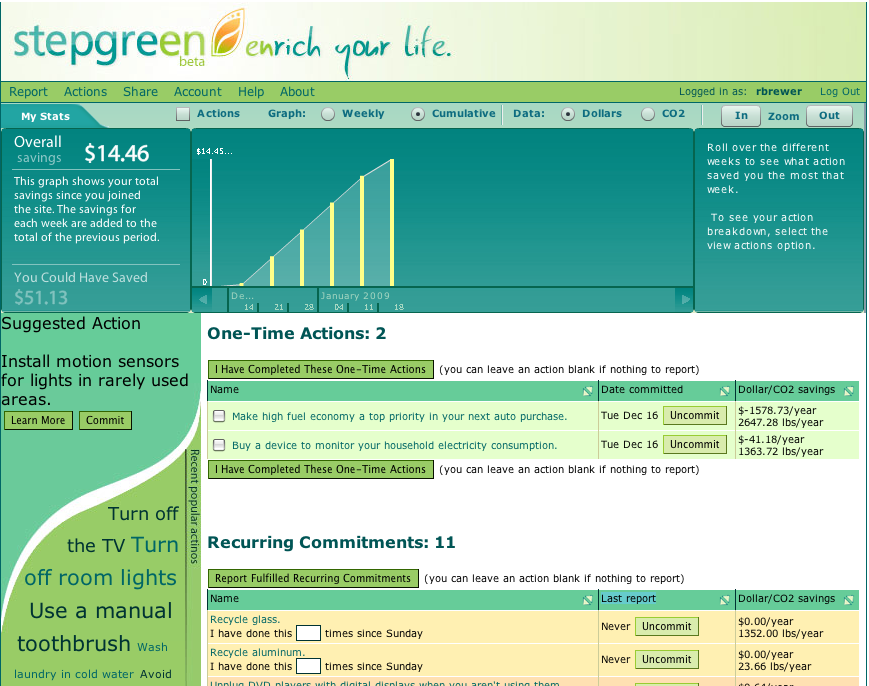
\includegraphics[width=\textwidth]{stepgreen-bitmap}
		\caption{Example page from StepGreen website}
		\label{fig:stepgreen-website}
\end{figure}

The StepGreen system is currently open to the public. \autoref{fig:stepgreen-website} shows an example of the default page shown when a user logs in. Users create an account on StepGreen, and then are presented with a list of actions with positive environmental consequences (mostly reduced GHG emissions). Example actions are ``Turn off the lights when you exit the house in the morning for the day'', ``Take the stairs at work'', and ``Set your home computer to automatically hibernate/sleep after a short period of inactivity''. Each action is associated with its cost savings and reduction in \COtwo emissions. Users can get more information about the action and how the savings were calculated. For each action, users can indicate whether they are already performing that action, whether they commit to undertaking that action, or whether the action is not applicable to them. Users can create new actions to be added to the list, but since the new actions have not been analyzed by the site maintainers, the financial and \COtwo savings are listed as unknown.

Once users have selected actions that they are either already performing or commit to performing, they can track them on the Reporting page. For one time actions, such as replacing an incandescent light bulb with a compact florescent bulb, users simply check off when they are completed. For recurring actions, users must indicate how many times they have performed the action since their last report in order for the system to track the activities. Based on the user's self-reporting, StepGreen calculates the amount of money saved, pounds of \COtwo saved (i.e., reduced), and missed pounds of \COtwo saved, and provides a historical graph of these values.

StepGreen also provides links to social networking sites. They provide a MySpace profile widget, and a connection to Twitter. Both of these links provides a way to inform the user's social network about what actions the user is undertaking. This feature can serve to recruit other people to use StepGreen, provide comparisons on financial and environmental savings among peers, and encourage users to keep to their StepGreen commitments. Mankoff et al.\ performed a field evaluation of StepGreen using 32 participants from the local community. Participants were asked to use the system over the three week period, and view their MySpace profile twice a day. The MySpace profile widget showed a graph of recent \COtwo or financial savings, recent commitments, and a new action suggestion. The goal of the evaluation was to analyze the usability of StepGreen, rather than the behavioral impact of the system. Participants committed to an average of 16 actions, and reported completing 88\% of the actions they committed to. Most participants reported that they learned about new actions through the evaluation, and almost half indicated that they now realized that household energy use was more of a factor in global warming than they had previously thought.

As a result of their evaluation, Mankoff et al.\ redesigned StepGreen to include more social features directly in StepGreen (such as comparison of data and discussion groups) rather than just piggybacking on existing social networks like MySpace. Manual reporting of actions was a participant concern, so the reporting page has been improved, and there are plans to support the input of sensor data from the UbiGreen transportation sensing project~\cite{Froehlich2009-ubigreen}. To deliver visualizations appropriate to different contexts such as a social media widget and the StepGreen website, StepGreen now supports an API that visualizations can query for data. An example visualization uses a virtual polar bear to motivate users to reduce their carbon footprint (see \autoref{sec:virtual-polar-bear}).

Grevet et al. studied social visualizations in StepGreen with a dorm competition at Wellesley College~\cite{Grevet10}. While the social visualization was received well, participants found that the list of actions in StepGreen was not well suited to their residence hall lifestyle.

StepGreen would be challenging to keep up to date due to the reliance on manual data input. Due to the limitations of manual reporting, StepGreen may report missed savings that are not accurate, annoying users. For example, recycling glass is an action that is listed as having substantial carbon savings. However, if one chooses to drink water from a mug instead of purchasing a beverage and later recycling the glass container, clearly the carbon savings are greater from using the mug, but StepGreen will count the lack of recycling as missed savings.


\subsection{Virtual Polar Bear}
\label{sec:virtual-polar-bear}

Dillahunt et al.\ (who are involved with the StepGreen project) have built a system providing a virtual polar bear that is affected by the user's environmental choices as a means to motivate users to reduce their carbon footprint \cite{dillahunt-virtual-polar-bear-2008}. They note that there are strong emotional bonds between humans and animals, which may help to encourage environmentally-responsible behavior. The authors performed a one week study, with subjects divided into two groups: an attachment group and a control group. The attachment group read a story about climate change impacting polar bear habitats, and were asked to name their virtual polar bear. As participants make or decline commitments to environmentally responsible actions, the ice under polar bear either grows or shrinks (see \autoref{fig:virtual-polar-bear} for images of the polar bear). The study had 20 subjects (10 for each group), all of whom were surveyed before and after to test for levels of empathy and environmental concern. The subjects in the attachment group had more fulfilled environmental commitments, which was a statistically significant difference. The attachment subjects also had a greater level of environmental concern after interacting with the polar bear. The authors were unsure whether effects would be sustained in a longer study. They are now working on bringing the system to a mobile platform and creating a polar bear application for Facebook and MySpace.

\begin{figure}[htbp]
	\centering
		\includegraphics{virtual-polar-bear}
		\caption{Example images of virtual polar bear with lots of ice and with little ice}
		\label{fig:virtual-polar-bear}
\end{figure}


\subsection{Personal Kyoto}
\label{sec:personal-kyoto}

Personal Kyoto is a web service that tracks the electricity usage of users in the New York area, and compares it to a ``Personal Kyoto Goal'' for the user \cite{Personal-Kyoto-website}. The Personal Kyoto Goal represents the limit of electricity usage that would apply to the user if the Kyoto Protocol (which the USA is not a party to) were administered on an individual basis rather than on a national basis.

The user's electricity usage is retrieved from the local utility's web site (Con Edison) using the user's account number. In addition to the monthly usage (which can vary substantially due to circumstances and the seasons), a 12 month rolling average is computed to remove the seasonal effects. The Personal Kyoto Goal is defined as 75\% of the first point of the monthly rolling average when the user signed up with the web site. \autoref{fig:personal-kyoto} shows an example graph with monthly averages and a personal Kyoto goal.

\begin{figure}[htbp]
	\centering
		\includegraphics[width=\textwidth]{personal-kyoto}
		\caption{Example graph of electricity usage from Personal Kyoto}
		\label{fig:personal-kyoto}
\end{figure}

Personal Kyoto is a cleverly designed system in that it uses the user's real data, but avoids manual data entry by scraping the data from the utility web site. It also gives the user a specific goal for reducing electricity use that has a real justification and ties into the environmental ``gravitas'' of the Kyoto Protocol.

\subsection{EcoIsland}
\label{sec:ecoisland}

Takayama and Lehdonvirta have constructed a system they call EcoIsland, which attempts to ``motivate behaviour changes that reduce CO2 emissions'' using a background game-like activity, with a centrally installed display in the home \cite{takayama-2008}. \autoref{fig:ecoisland} shows an example of the user interface. Each family member has an avatar on the virtual island, and they set a family \COtwo emissions target. The family's emissions are tracked via sensors and self-reporting. If the emissions exceed the chosen target level, the water level on the island rises, and if the water level continues to rise it will eventually end the game.

\begin{figure}[htb]
	\centering
		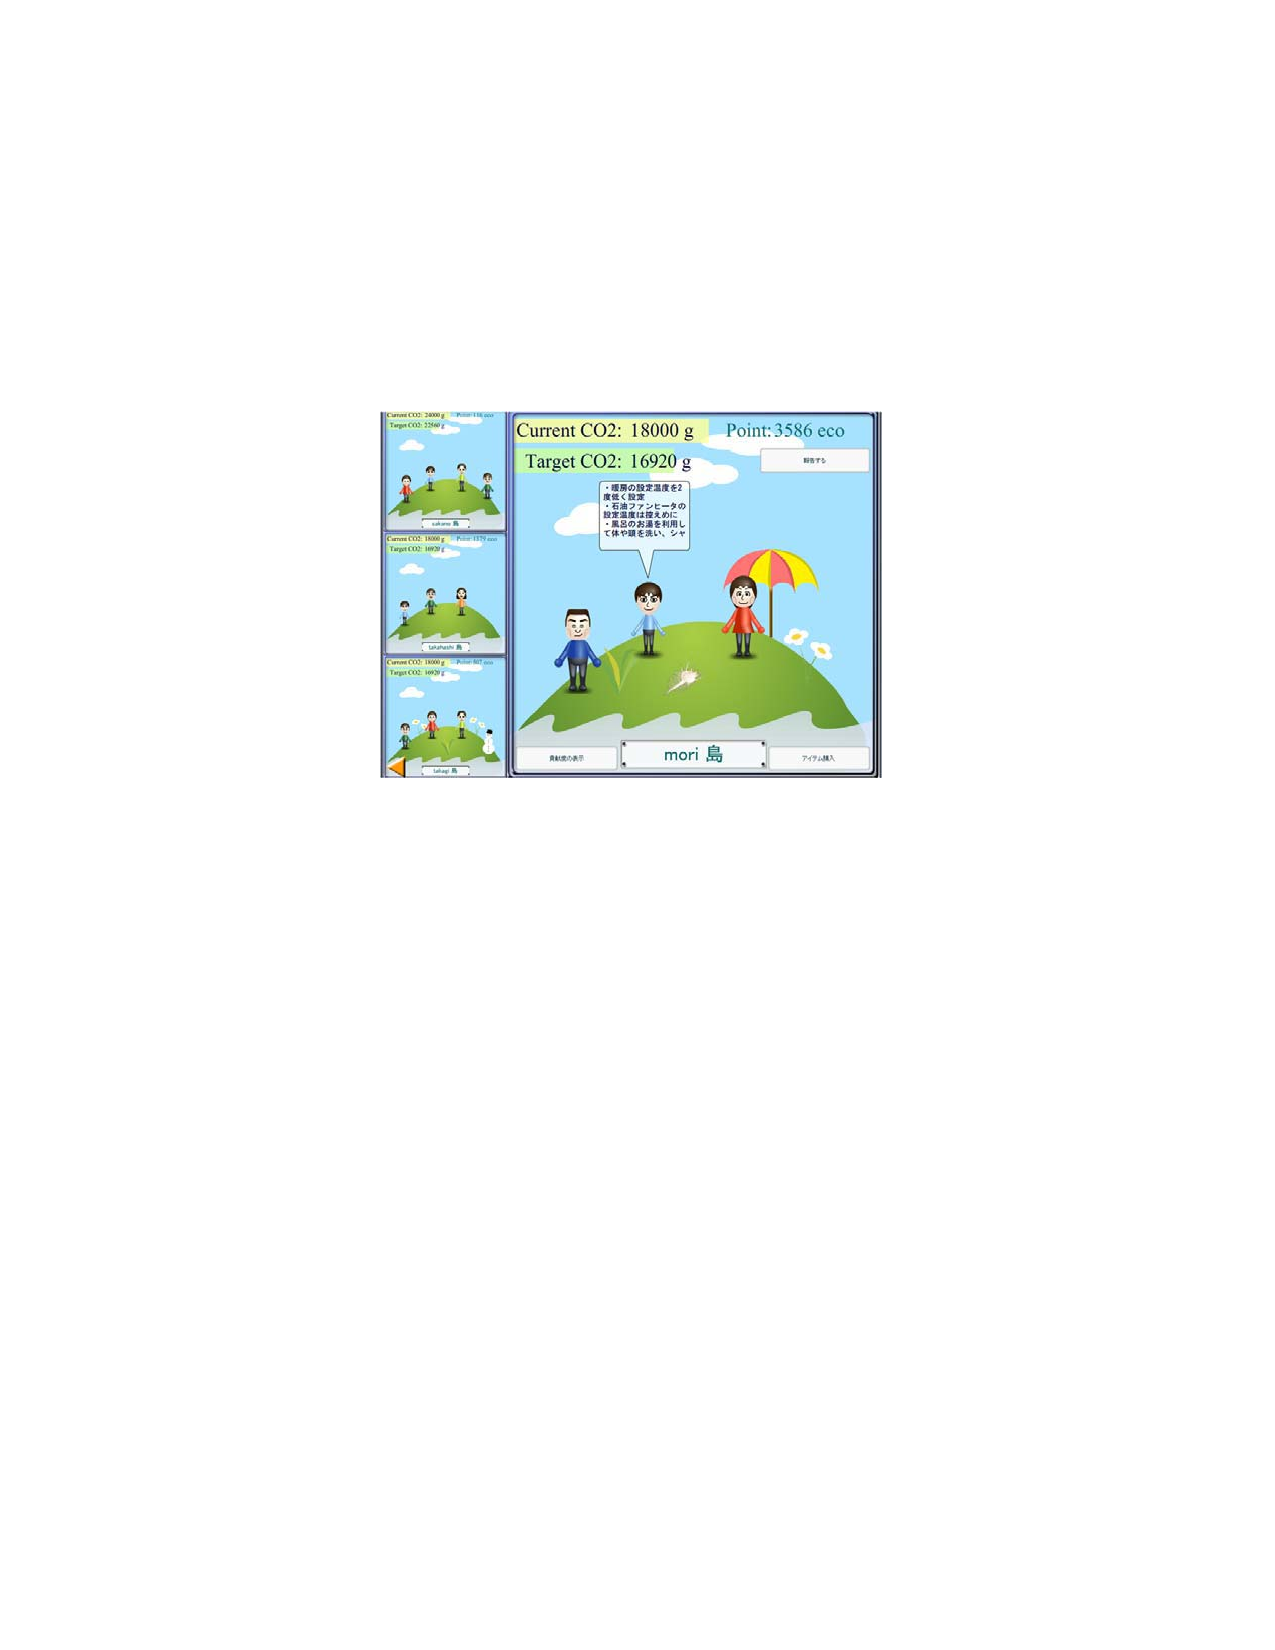
\includegraphics[width=0.8\textwidth]{ecoisland}
		\caption{Example EcoIsland display, with family avatars}
		\label{fig:ecoisland}
\end{figure}

Participants mobile phones have a list of suggested actions to reduce emissions, and they can self-report their actions using the phone. Participants can see the islands of other participants and they receive a periodic allowance in a virtual currency. The participants can use the virtual currency to buy decorations for their island, or to purchase carbon credits from other users. Participants with low emissions, therefore, can decorate their island, while those with high emissions have to spend their money on carbon credits. EcoIsland provides a metaphor for the users' emissions and makes them aware of the consequences of their actions.

The sensor portion of the system was not yet implemented at the time the authors conducted their study. The authors performed a four week pilot study of EcoIsland with 20 people in six families. During the first week, the baseline electricity usage of each participant's air conditioning system was monitored using a plug load meter (for more information on this type of meter, see \autoref{sec:plug-load-meters}). During the second week, one participant from each household was asked to use the system, while in the third week all members were asked to use it. In the fourth week, the carbon trading system was introduced to participants. At the conclusion of the study, the participants were surveyed and 17 of 20 participants said ``they were more conscious of environmental issues after the experiment than before.'' However, users indicated that they were motivated by game issues (such as saving the sinking island and buying in-game decorations) rather than saving the environment. Few of the participants used the carbon trading system because their targets were easy enough to achieve without trading. Air conditioner usage in participant homes showed no correlation with game outcome, but the authors believe that the short study may have affected that outcome. The study was conducted in winter, which might seem like an inappropriate time to measure air conditioner use. However, in Japan, many air conditioning units also function as heaters, so it may be this type of air conditioner usage that the authors are referring to. One interesting result is that participants noted that manual reporting contributed to their motivation, so replacing the reporting with sensors could reduce user's motivation to change.


\subsection{PowerHouse}

Reeves et al.\ have developed an online game called Power House intended to use the engagement of games to encourage players to reduce their energy usage~\cite{Reeves2011powerhouse}. Power House players import their electricity use data from their utility (recorded by smart meter). The game dashboard shows recent electricity usage, and real-world electricity usage impacts the results of the online games. Multiple online mini-games are provided for players, such as a game where players move around a house, turning on and off appliances to allow their in-game avatars to complete actions such as washing clothes or cooking dinner. Players that have conserved energy in their actual homes are able to turn on more appliances in their virtual home before tripping a circuit breaker, making game play easier. Power House is being evaluated, but results are not yet available. Power House is similar to the Kukui Cup in its integration of real-world and online actions, but Power House contains professional-quality mini-games, while the Kukui Cup focuses on educational actions both online and in the real world.


\subsection{Google PowerMeter}
\label{sec:google-powermeter}

Utilities are starting to install `smart meters' (also called AMI for Advanced Metering Infrastructure) on homes as part of an overall push towards the `smart grid'. However, these smart meters are often thought about from the utility's perspective: eliminating manual meter reading, enabling time-of-day electricity pricing, and monitoring power reliability. While there are many benefits for the utility, frequently updated power data from the meter could be very useful if provided directly to the people being metered, as discussed in \autoref{sec:energy-feedback}.

Google PowerMeter is a web application developed to make smart meter data available to the end users living in smart metered homes \cite{Google-PowerMeter}. Google partners with utilities that have rolled out smart meters, and collects the power data from the utility. PowerMeter also works with the TED 5000 home energy meter that can be installed by end-users without interaction with the utility (see \autoref{sec:panel-meters}). The data is recorded at 15 minute intervals, and presented in a variety of graphs that show daily usage and home base load levels. \autoref{fig:google-powermeter} shows an example display for a home in \Hawaii. The primary interface for PowerMeter is a web gadget that is installed on the user's iGoogle home page. PowerMeter allows users to share their data with others, and has added an API to allow users to get access to their raw data. Google decided to shut down the PowerMeter service on September 16, 2011 because ``our efforts have not scaled as quickly as we would like''~\cite{PowerMeter-shutdown}.

\begin{figure}[htbp]
	\centering
		\includegraphics[width=\textwidth]{google-powermeter}
		\caption{Google PowerMeter data for a home in \Hawaii}
		\label{fig:google-powermeter}
\end{figure}

\subsection{Microsoft Hohm}

Microsoft Hohm is a web application that allows consumers to view their energy usage (similar to Google PowerMeter) and offers recommendations for energy conservation~\cite{MS-Hohm-website}. \autoref{fig:microsoft-hohm} shows an example display for a home in \Hawaii. For homes that do not have a utility-installed smart meter or a consumer-installed energy monitoring device, Hohm allows users to supply their address and characteristics of their home to estimate their energy use. Unfortunately, the default data Hohm provides for \Hawaii homes is inaccurate, as it assumes that all homes use energy for heating. Based on the energy data and home characteristics entered by the user, Hohm provides detailed suggestions for saving energy, such as lowering the temperature of water heaters, including cost saving and \COtwo emission savings. Like Google PowerMeter, Microsoft decided to discontinue the service ``due to the slow overall market adoption of the service''~\cite{Hohm-discontinued}. Hohm is scheduled to be shut down on May 31, 2012.

\begin{figure}[htbp]
	\centering
		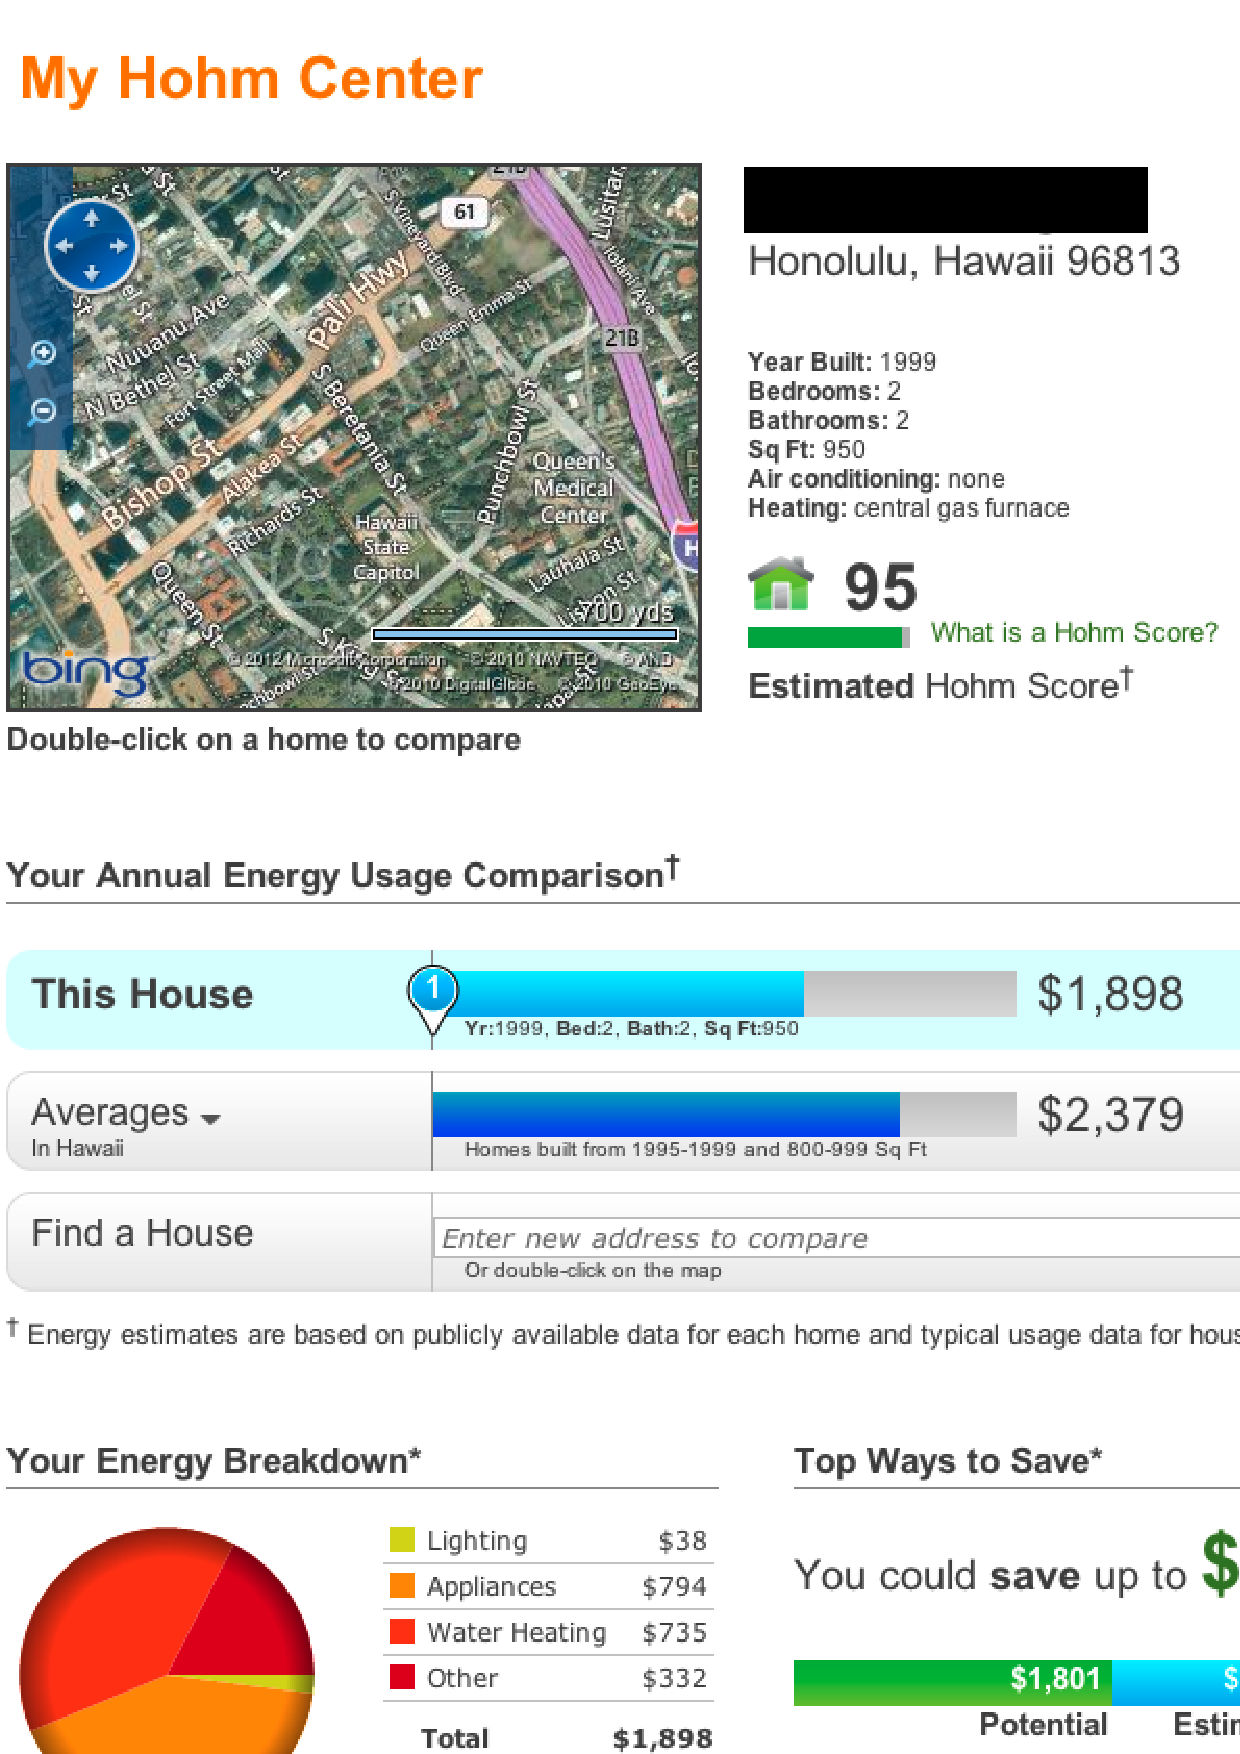
\includegraphics[width=\textwidth]{microsoft-hohm-crop}
		\caption{Microsoft Hohm data for a home in \Hawaii}
		\label{fig:microsoft-hohm}
\end{figure}


\subsection{iamgreen}
\label{sec:iamgreen}

iamgreen is an application for the Facebook social networking platform that provides an online gathering place for environmentally conscious users \cite{iamgreen-website}. iamgreen provides all of the standard components of Facebook: a newsfeed of events from members, status updates, news articles, etc. The application provides a list of environmentally responsible statements called ``leaves'', such as ``Most of my lightbulbs are compact fluorescents'', ``I recycle, even when it is not convenient'', and ``When I drive, it's over 40mpg baby'' (see \autoref{fig:iamgreen} for an example of the leaf selection page). For each statement, users can indicate if they engage in that behavior, they aspire to that behavior, they wish to hide the statement (removing it from the list of choices), or they want to recommend it to a friend. Users can then display the number of leaves they have committed to in their Facebook profiles. Users can also contribute new leaves, which will be displayed as options to other iamgreen users.

\begin{figure}[htbp]
	\centering
		
\includegraphics[width=0.8\textwidth]{iamgreen}
		\caption{Leaf selection page of iamgreen Facebook application}
		\label{fig:iamgreen}
\end{figure}

While the leaves concept is a simple way to encourage users to make more environmentally positive choices, it suffers from some obvious deficiencies. First, leaves, for the most part, have the same value (though apparently some actions, such as not owning a car, are worth more than one leaf). The leaf system also lacks any quantitative feedback other than the number of leaves, so the user is not provided with real insight into their environmental footprint. Like any system based on manual reporting, users have to spend time reporting any changes to their action list. Without quantitative feedback, it seems likely that many users will make some selection of leaves and then revisit them infrequently or never again.


\section{Dormitory Energy Competitions}
\label{sec:dorm-energy-competitions}

Residence hall energy competitions are events where residence halls or floors within a residence hall compete to see which building will use the least energy over a period of time. Some competitions pull in other aspects of environmental sustainability, including reducing water usage, reduced waste production, etc. The competitions tap into both the residents competitive urges, and the interest in environmental issues. However, unlike a home environment, the residents typically do not financially benefit from any reduction in electricity use resulting from their behavior changes, since residence hall fees are flat-rate and do not change based on energy usage. This leads to residents being completely unaware of their energy usage, since they lack even a monthly bill as feedback. Dillahunt et al. describe similar a similar situation with their investigation of energy usage in low income communities, where individuals may not be billed directly for electricity and may not have the means to upgrade appliances~\cite{Dillahunt2009-low-income}. Despite these differences, Dillahunt et al. found that the residents of low-income housing were still motivated to save energy and came up with diverse energy-saving solutions, which may suggest that dorm residents can be similarly motivated.

Energy competitions in residence halls have become a popular event at colleges and universities: in 2010, a survey by Hodge found 163 colleges that had held a dorm energy competition or planned to during the 2010--2011 academic year~\cite{Hodge2010}, with approximately 40\% of schools running their first competition in 2008 or later.

The most basic type of energy competition website displays energy data which is updated manually on a periodic basis (such as weekly). The Wellesley College Green Cup \cite{wellesley-green-cup} is an example of this type of competition.

\subsection{Oberlin College Energy Competition}

Other schools have more complicated and interactive competition websites, such as the early adopter Oberlin College. Petersen et al.\ describe their experiences deploying a realtime feedback system in an Oberlin College dorm energy competition in 2005 \cite{petersen-dorm-energy-reduction,Petersen07a}. 22 dormitories were in competition over a 2 week period, with 2 dorms having feedback updates every 20 seconds, and the other 20 getting updates every week. The realtime dorms also recorded electricity usage for each of the three floors, but only displayed the data from two of the floors, leaving the third as a control. Web pages were used to provide feedback to students, since they all have computers and Internet access in their rooms. They found a 32\% reduction in electricity use across all dormitories, with the 2 realtime feedback dorms reducing usage the most. Freshman dorms were among the highest electricity reducers, while upperclassman dormitories were quite low (average 2\% reduction). During a 2 week post-competition period, the average electricity usage was similar to consumption levels during the competition. However, the weather was warmer and there was more sunlight during the post-competition period, so it is unclear if the reduction was competition-related.

In terms of participation, Petersen et al.\ found 46\% of residents looked at the competition website at least once (based on web server logs mapping IP addresses to residence halls). 23\% of dormitory residents filled out the online post-competition survey. Survey respondents indicated that some behaviors, such as turning off hallway lights at night and unplugging vending machines were not sustainable outside the competition period.

\subsection{Campus Conservation Nationals}

The Campus Conservation Nationals (CCN) is a series of energy and water use reduction competitions run in residence halls on college campuses in 2010 and 2012~\cite{conservation-nationals-2012}. 40 schools participated in the 2010 pilot competition, with a claim of 508,000\kWh saved due to the competition. There are 150 schools participating in the 2012 competition (taking place between February 6 until April 23), with a goal of one gigawatt-hour of energy savings for all schools combined. Both the 2010 and 2012 competitions lasted three weeks, though in 2012 each school could pick which three weeks to run the competition during the 11 week window~\cite{conservation-nationals-website}. Each school was allowed to decide what baseline values to use for each residence hall, with a suggestion to use the average energy and water consumption for the hall over the two weeks prior to the competition. The baselines are not normalized for changes in weather during the competition or between competing schools. The energy and water use data is manually input by each school at least once per week during the competition, but the organizers request that it not be input more frequently than once every two days. Each school can choose to compete in different ways: competitions among residence halls on a single campus, competitions among schools in a geographic region, and competitions among peer institutions. Each school is responsible for providing prizes to the residence hall that conserved the most energy and/or water, while the national sponsors provide prizes to the schools that reduce the most overall. There does not appear to be any measurement of energy or water use after the competition is over, though there is a web questionnaire for students that schools can direct their participants to, with the data being collected by researchers at Oberlin College.

\subsection{Western Washington University Go for Green Challenge}

Western Washington University held a Go for Green Challenge in 2008, described in a Masters thesis by Mauney~\cite{Mauney-thesis}. The challenge took place in eight of sixteen on-campus residence halls, with the remaining eight halls serving as a comparison group. The competition took place over three months from January 8 to April 1, 2008. A survey of residents in advance of the competition showed low participation rates in residence hall activities: 80\% reported that they do not participate at all in such activities. The goals of the challenge were to reduce electricity use by 10\%, and increase energy awareness and participation by residents. Energy use was measured using building-level meters that were recorded once per month. The residence halls all had different construction and numbers of residents, so the energy use was compared to a baseline for each hall and normalized to kilowatt-hours per resident. Three monthly baselines were computed for the three months of the competition by averaging the number of kilowatt-hours used by the hall for that month in the previous three years (2005--2007). To encourage participation, the challenge each hall earned points by the actions of their residents. Each 1\% energy reduction that a hall made from the baseline was worth 20 points, while each resident that made a green pledge, completed a survey, or attended a hall event earned 1 point for their hall. Prizes donated by local businesses were awarded to the halls that earned the most points. To organize and promote the challenge in each hall, leaders were recruited, including: Resident Advisors (RAs), Resident Directors (RDs), and EcoReps (residents recruited to help run the competition). The leaders were encouraged to take initiative in planning events and promoting the challenge, so the experience of residents in each hall was different. The treatment halls where the challenge ran were not randomly selected: only halls that had EcoReps or involved RDs were selected, leading to a quasi-experimental design.

A survey was administered to residents of all participating halls before, midway through, and after the challenge to assess attitudes towards conservation, behavior changes, and education. The survey had several sections:

\begin{itemize}
	\item Classifying fellow hall residents as: conservers, efficient users, unaware, or overly consumptive
	\item Frequency of six self-reported behaviors around elevator use, turning off devices, and shower use
	\item Education question (did you learn something as result of challenge): yes or no
\end{itemize}

The responses between the different surveys were not matched up within subjects, and the comparison halls were not surveyed.

Mauney found that treatment halls showed greater energy reduction compared to the baseline than comparison halls. However, 7 of the 8 comparison halls showed reduction in energy use during the GGC. Average energy reduction in treatment halls was 12.5\%, and 6.1\% for comparison halls. Since the baseline was computed using three years of historical data, some hall reductions were believed to be caused by renovations that improved the hall's energy efficiency, but other halls had no recent renovations.

The pre-challenge survey had a response rate of 18\%, while the post-challenge survey had an 11\% response rate. Mauney found that the survey response rate was significantly correlated with the percentage of hall residents that signed the green pledge. Reduction in energy use was significantly correlated with percentage of residents classified as conservers or efficient users. As expected, halls that had interior hallways with more chances for resident interaction reduced more than apartments with exterior hallways. There were small changes in reported behavior pre and post challenge, including more unplugging appliances and lower elevator usage.

In addition to the resident questionnaire, the challenge leaders (RAs, RDs, EcoReps) were surveyed about their experiences after the first month of the competition. Leaders were asked how they communicated about the challenge to residents, and what behavior changes they observed in their residents. The most common promotion strategies were posted materials, and verbal discussion including going door to door in the hall. The largest behavior change in residents noted by leaders was turning out lights when not in use.

Mauney concludes that having RAs or EcoReps in each hall is an important factor for success in the challenge: the best performing hall had an RD who made the challenge the main program focus during the challenge period. RDs also wished to see some of the money saved by the energy reduction returned to halls, but this is complicated by uncertainty in whether the reduction was due to behavior change or other factors.

The Go for Green Challenge has many similarities to the Kukui Cup: a point system to motivate participants, addition of energy education, and pre and post challenge surveys of participants. However, it had several shortcomings: no individual points, monthly energy use feedback, limited program activities, no web interface, and a problematic multi-year baseline calculation. The 2011 Kukui Cup addressed each of these issues.


\subsection{Dorm Energy Competition Survey}

Hodge's survey of dorm energy competitions found a wide range of energy conservation results from the competitions~\cite{Hodge2010}. The median competing building reduced energy use by 9\%, but the worst building increased usage by 12\%. The median winning building reduced by 22\%, but the worst winning building was 0\% and the best was 80\%! Hodge identifies five core components of dorm energy competitions:

\begin{itemize}
	\item Incentives, such as food, parties, and trophies
	\item Team-based competition instead of individual competition
	\item Short competitions lasting approximately one month
	\item Energy feedback, including ranking compared to other dorms
	\item ``Hype'', such as dances and cafeteria meals lit by candlelight
\end{itemize}


\subsection{Dorm Energy Competition Summary}

The Oberlin energy competitions, with their real-time energy feedback, were a major influence on the design of the 2011 Kukui Cup. The idea of metering floor-by-floor in the Kukui Cup, rather than building-by-building was intended to build more tightly-knit teams, and allow the effects of behavior change to be more apparent since the feedback would occur on a smaller scale. The WWU Go for Green Challenge has several similarities to the Kukui Cup. In both competitions, points could be earned as well as energy conserved, though in the Kukui Cup individuals could earn points and the energy competition was not directly linked to the point competition. The Go for Green challenge also used survey instruments before and after the competition, though subjects were not matched across the surveys as they were in the Kukui Cup. Mauney's suggestion that involved RAs and EcoReps are important to the success of the competition is well-heeded, though we did encounter some difficulties in this area (see \autoref{sec:ra-participation}). Regarding Hodge's five components for a successful energy competition, the 2011 Kukui Cup incorporated each of the five components.


% \section{Does Energy Efficiency Reduce Carbon Emissions?}
% \label{sec:efficiency-rebound}
% 
% Many governmental plans to reduce GHG emissions involve improving energy efficiency in the home, in industry, and in transportation. While intuitively it would seem that increased energy efficiency would lead to decreased energy usage, and thereby reduced GHG emissions, surprisingly there is some evidence (both theoretical and empirical) that energy efficiency actually increases energy usage! Saunders dubbed this unintuitive notion the Khazzoom-Brookes Postulate based on conclusions reached independently by those two researchers \cite{saunders-1992}. \fxnote{Insert references to Khazzoom and Lovins papers here, after I read them.}
% 
% Using neoclassical growth theory, Saunders finds that increased energy efficiency makes energy seem cheaper, thus allowing it to be substituted for labor in production. Increased energy efficiency also increases overall economic growth, which leads to increased overall energy usage.
% 
% In discussing this effect, rebound is defined as the difference between the expected amount of energy savings from an improvement in energy efficiency, and the actual observed effect. For example, if an improvement in metal smelting technology reduces the energy required to smelt by 20\%, but the energy consumed by the metal smelting industry only goes down by 10\% then the rebound is 50\%. If the rebound is greater than 100\%, then backfire is taking place (the efficiency measure has backfired) \cite{Hanley2008Do-increases-in}. There is some debate over whether the predicted increases in energy usage will actually take place in the real world. Laitner suggests via a simple analysis that the rebound effect is small (2.4\%) \cite{Skip-Laitner:2000yg}. His equation relates future carbon emissions to current carbon emissions, increases in GDP and energy costs, and elasticities of income and energy prices to arrive at this conclusion. He goes on to a further analysis done by the Environmental Protection Agency and Lawrence Berkeley National Labs using the National Energy Modeling System showing that an ``energy-efficient/low-carbon technology path'' would suffer from a rebound effect of only 2.2\%. However, he acknowledges that consumer choices about energy usage could erode gains from efficiency, such as turning up the furnace thermostat because the cost of doing so has been effectively reduced.
% 
% The issue of consumer choices is a real one. Over the last 25 years, automobiles have been made more efficient through ``increasing the efficiency of the engine and transmission, decreasing weight, improving tires and reducing drag'' \cite{Heywood2008Fueling-Our-Future}. However, these improvements have been traded for vehicles that are larger, heavier, and faster, which has led to only modest improvements in overall fuel efficiency. This is an example of how energy efficiency may not always lead to reduced GHG emissions without motivating automobile users (and manufacturers) to buy and make fuel efficient vehicles.
% 
% Other authors find that rebound and even backfire are the likely results of economy-wide improvements in energy efficiency. The analysis of Hanley et al. finds that backfire occurs when economy-wide improvements in energy efficiency are made \cite{Hanley2008Do-increases-in}. Their theoretical analysis finds that if energy demand is relatively price-elastic (demand increases when prices are low and decreases when prices are high), then backfire will occur. Empirical evidence of rebound and backfire are hard to come by because there are indirect system-wide effects due to the increased efficiency, and these indirect effects are difficult to measure. The authors created a Computable General Equilibrium (CGE) model of Scotland that simulates the economy and environmental impact based on the inputs and outputs of the system. Using this model, almost all scenarios eventually result in backfire. They note that since non-renewable energy sources use more energy in their production than renewable sources, increased energy efficiency lowers the cost of non-renewables compared to renewables, financially favoring the use of non-renewables. Efficiency in energy production is therefore associated with a decrease in the use of energy from renewable sources. The authors also urge caution when reviewing sustainability measures such as the ratio of Gross Domestic Product (GDP) to energy usage or carbon emissions, because even if the ratio increases (less carbon per unit GDP), if the GDP as a whole increases faster, the absolute carbon emitted will increase. They suggest that backfire could be prevented by combining energy efficiency improvements with taxes on energy use or a carbon tax. Since energy efficiency effectively reduces the cost of energy, the savings could offset the cost of additional taxes, thereby blunting any impact on economic activity.
% 
% It would appear that any energy efficiency improvements will have some degree of rebound effect, thus a naive pursuit of energy efficiency without taking into account the context around the improvements could risk reducing their effectiveness, or even making them counterproductive! While many of the analyses deal at the macroeconomic level, it is not hard to think of individual scenarios where efficiency could actually increase personal usage, such buying two energy efficient refrigerators to replace one older energy-hogging refrigerator. The key to ensuring that energy efficiency improvements on the micro level lead to less GHG emissions is to combine efficiencies with changes in behavior.
